% Options for packages loaded elsewhere
\PassOptionsToPackage{unicode}{hyperref}
\PassOptionsToPackage{hyphens}{url}
%
\documentclass[
  man,floatsintext]{apa6}
\usepackage{lmodern}
\usepackage{amssymb,amsmath}
\usepackage{ifxetex,ifluatex}
\ifnum 0\ifxetex 1\fi\ifluatex 1\fi=0 % if pdftex
  \usepackage[T1]{fontenc}
  \usepackage[utf8]{inputenc}
  \usepackage{textcomp} % provide euro and other symbols
\else % if luatex or xetex
  \usepackage{unicode-math}
  \defaultfontfeatures{Scale=MatchLowercase}
  \defaultfontfeatures[\rmfamily]{Ligatures=TeX,Scale=1}
\fi
% Use upquote if available, for straight quotes in verbatim environments
\IfFileExists{upquote.sty}{\usepackage{upquote}}{}
\IfFileExists{microtype.sty}{% use microtype if available
  \usepackage[]{microtype}
  \UseMicrotypeSet[protrusion]{basicmath} % disable protrusion for tt fonts
}{}
\makeatletter
\@ifundefined{KOMAClassName}{% if non-KOMA class
  \IfFileExists{parskip.sty}{%
    \usepackage{parskip}
  }{% else
    \setlength{\parindent}{0pt}
    \setlength{\parskip}{6pt plus 2pt minus 1pt}}
}{% if KOMA class
  \KOMAoptions{parskip=half}}
\makeatother
\usepackage{xcolor}
\IfFileExists{xurl.sty}{\usepackage{xurl}}{} % add URL line breaks if available
\IfFileExists{bookmark.sty}{\usepackage{bookmark}}{\usepackage{hyperref}}
\hypersetup{
  pdftitle={Mathematical study of Glass's d},
  pdfauthor={Marie Delacre},
  pdfkeywords={keywords},
  hidelinks,
  pdfcreator={LaTeX via pandoc}}
\urlstyle{same} % disable monospaced font for URLs
\usepackage{graphicx,grffile}
\makeatletter
\def\maxwidth{\ifdim\Gin@nat@width>\linewidth\linewidth\else\Gin@nat@width\fi}
\def\maxheight{\ifdim\Gin@nat@height>\textheight\textheight\else\Gin@nat@height\fi}
\makeatother
% Scale images if necessary, so that they will not overflow the page
% margins by default, and it is still possible to overwrite the defaults
% using explicit options in \includegraphics[width, height, ...]{}
\setkeys{Gin}{width=\maxwidth,height=\maxheight,keepaspectratio}
% Set default figure placement to htbp
\makeatletter
\def\fps@figure{htbp}
\makeatother
\setlength{\emergencystretch}{3em} % prevent overfull lines
\providecommand{\tightlist}{%
  \setlength{\itemsep}{0pt}\setlength{\parskip}{0pt}}
\setcounter{secnumdepth}{-\maxdimen} % remove section numbering
\shorttitle{Glass's d}
\affiliation{
\vspace{0.5cm}
\textsuperscript{1} Université Libre de Bruxelles, Service of Analysis of the Data (SAD), Bruxelles, Belgium}
\keywords{keywords\newline\indent Word count: X}
\usepackage{csquotes}
\usepackage{upgreek}
\captionsetup{font=singlespacing,justification=justified}

\usepackage{longtable}
\usepackage{lscape}
\usepackage{multirow}
\usepackage{tabularx}
\usepackage[flushleft]{threeparttable}
\usepackage{threeparttablex}

\newenvironment{lltable}{\begin{landscape}\begin{center}\begin{ThreePartTable}}{\end{ThreePartTable}\end{center}\end{landscape}}

\makeatletter
\newcommand\LastLTentrywidth{1em}
\newlength\longtablewidth
\setlength{\longtablewidth}{1in}
\newcommand{\getlongtablewidth}{\begingroup \ifcsname LT@\roman{LT@tables}\endcsname \global\longtablewidth=0pt \renewcommand{\LT@entry}[2]{\global\advance\longtablewidth by ##2\relax\gdef\LastLTentrywidth{##2}}\@nameuse{LT@\roman{LT@tables}} \fi \endgroup}


\usepackage{lineno}

\linenumbers

\title{Mathematical study of Glass's d}
\author{Marie Delacre\textsuperscript{1}}
\date{}

\authornote{
I would like to thank Matt Williams and Thom Baguley for their helpful insights in order to undertand the phenomenon explained in this appendix.

Correspondence concerning this article should be addressed to Marie Delacre, CP191, avenue F.D. Roosevelt 50, 1050 Bruxelles. E-mail: \href{mailto:marie.delacre@ulb.ac.be}{\nolinkurl{marie.delacre@ulb.ac.be}}}

\abstract{

}

\begin{document}
\maketitle

\hypertarget{when-two-samples-are-extracted-from-distributions-with-identical-shapes-with-sigma_1-sigma_2-and-n_1n_2}{%
\section{\texorpdfstring{When two samples are extracted from distributions with identical shapes, with \textbf{\(\sigma_1= \sigma_2\)} and \textbf{\(n_1=n_2\)}}{When two samples are extracted from distributions with identical shapes, with \textbackslash sigma\_1= \textbackslash sigma\_2 and n\_1=n\_2}}\label{when-two-samples-are-extracted-from-distributions-with-identical-shapes-with-sigma_1-sigma_2-and-n_1n_2}}

When population distributions are symmetric (i.e.~\(\gamma_1=0\)), the sampling distribution of glass's \(d_s\) is the same, whatever one chooses \(s_1\) or \(s_2\) as standardizer. As an example, in Figure \ref{fig:glass1}, we plotted the sampling distribution of both measures of glass's \(d_s\) when two samples of 20 subjects are extracted from two symmetric distributions where \(\gamma_1=0\),\(\gamma_2=95.75\), \(\sigma_1=\sigma_2=1\) and \(\mu_2=0\). \(\mu_1\) is either 0 or 1, depending on the plot. One can see that in the two plots, distributions of glass's \(d_S\) using \(s_1\) and \(s_2\) as standardiser are superimposed. \footnote{Anytime the mean difference is null, the sampling distribution of glass will be symmetric. On the other side, anytime the mean difference is non null, the sampling distriution of glass's ds will be skewed: right-skewed if the mean difference is positive, left-skewed if the mean difference is negative. The right skewed distribution is therefore only due to the sense of the mean difference}

\begin{figure}
\centering
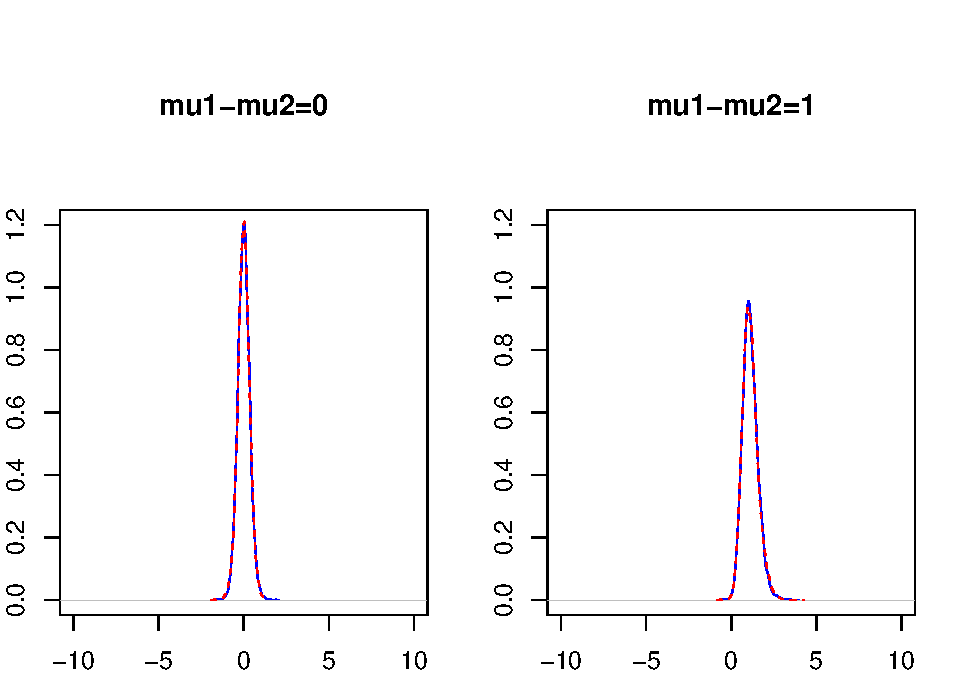
\includegraphics{Mathematical-study-of-Glass-s-d_files/figure-latex/glass1-1.pdf}
\caption{\label{fig:glass1}Comparison of Glass's ds when choosing either s1 (blue line) or s2 (red dotted line) as standardizer, with s1=standard deviation of the first sample and s2=standard deviation of the second sample, when n1=n2=20 and both samples are extracted from a distribution where G1 =0, G2=95.75 and sigma=1}
\end{figure}

However, when population distributions are skewed (i.e.~\(\gamma_1 \neq 0\)), the sampling distribution of glass's \(d_s\) varies as a function of the chosen standardizer, as illustrated in Figure \ref{fig:glass2}.

\begin{figure}
\centering
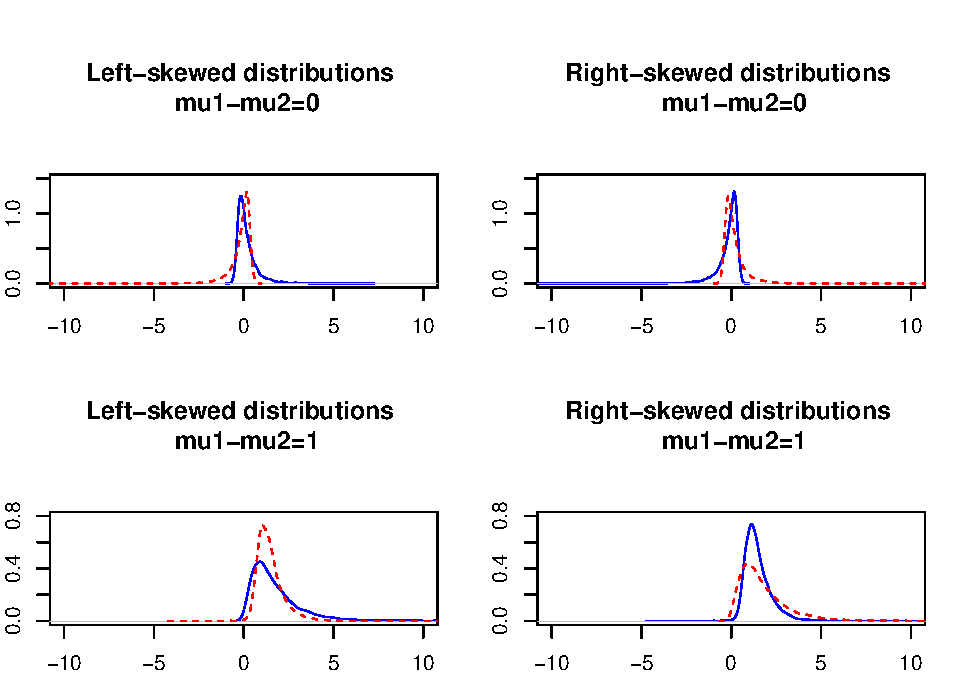
\includegraphics{Mathematical-study-of-Glass-s-d_files/figure-latex/glass2-1.pdf}
\caption{\label{fig:glass2}Comparison of Glass's ds when choosing either sd1 (blue line) or sd2 (red dotted line) as standardizer when n1=n2=20 and both samples are extracted from a distribution where sigma=1, G2=95.75, G1 is either -6.32 (left) or 6.32 (right). In all cases, the second sample is extracted from a population distribution where mu2=0. First sample is extracted from a population distribution where mu1 is either 0 (top) of 1 (bottom)}
\end{figure}

It might seem surprising, or even counter-intuitive, as in all plots, \(s_1\) and \(s_2\) are both estimates of the same population standard deviation (\(\sigma\)), based on the same number of observations (as \(n_1=n_2\)), but this phenomenon can be mathematically explained. In the following section, we will provides detailed informations to understand the results plotted in Figure \ref{fig:glass2}.

\hypertarget{when-both-samples-are-extracted-from-a-common-right-skewed-distribution-mu_1-mu_20-top-right-plot-in-figure}{%
\subsection{\texorpdfstring{When both samples are extracted from a common right-skewed distribution (\textbf{\(\mu_1-\mu_2=0\)}) (top right plot in Figure \ref{fig:glass2})}{When both samples are extracted from a common right-skewed distribution (\textbackslash mu\_1-\textbackslash mu\_2=0) (top right plot in Figure )}}\label{when-both-samples-are-extracted-from-a-common-right-skewed-distribution-mu_1-mu_20-top-right-plot-in-figure}}

We will first study the configuration where both samples are extracted from a right-skewed distribution where \(\mu=0\), \(\sigma=1\), \(\gamma_1=6.32\) and \(\gamma_2=95.75\). Because this distribution is right-skewed, the sampling distributions of \(\bar{X_1}\) and \(\bar{X_2}\) will also be right-skewed. However, because \(\bar{X_1}\) and \(\bar{X_2}\) are identically distributed, \(\bar{X_1}-\bar{X_2}\) will follow a symmetric distribution, as illustrated in Figure \ref{fig:sampldist1} (right plot).
More specifically, the distribution will be symmetrically centered around \(\mu_1-\mu_2=0\) (i.e.~the green area in the right plot in Figure \ref{fig:sampldist1} is the reflexion of the blue area, with the vertical line being the line of reflexion). It means that:\\
- Half the mean difference estimates will be positive (i.e.~\(\bar{X_1}-\bar{X_2} > 0\); see green area ) and the other half will be negative (i.e.~\(\bar{X_1}-\bar{X_2} < 0\); see blue area).\\
- For a constant k, \(|(\mu_1-\mu_2)-k|=|(\mu_1-\mu_2)+k|\)

Because we compute the mean difference as the mean estimate of the first sample minus the mean estimate of the second sample, there is a positive correlation between \(\bar{X_1}\) and \(\bar{X_1}-\bar{X_2}\), and a negative correlation between \(\bar{X_2}\) and \(\bar{X_1}-\bar{X_2}\) (correlations would be trivially reversed if we computed \(\bar{X_2}-\bar{X_1}\) instead of \(\bar{X_1}-\bar{X_2}\)).

\begin{figure}
\centering
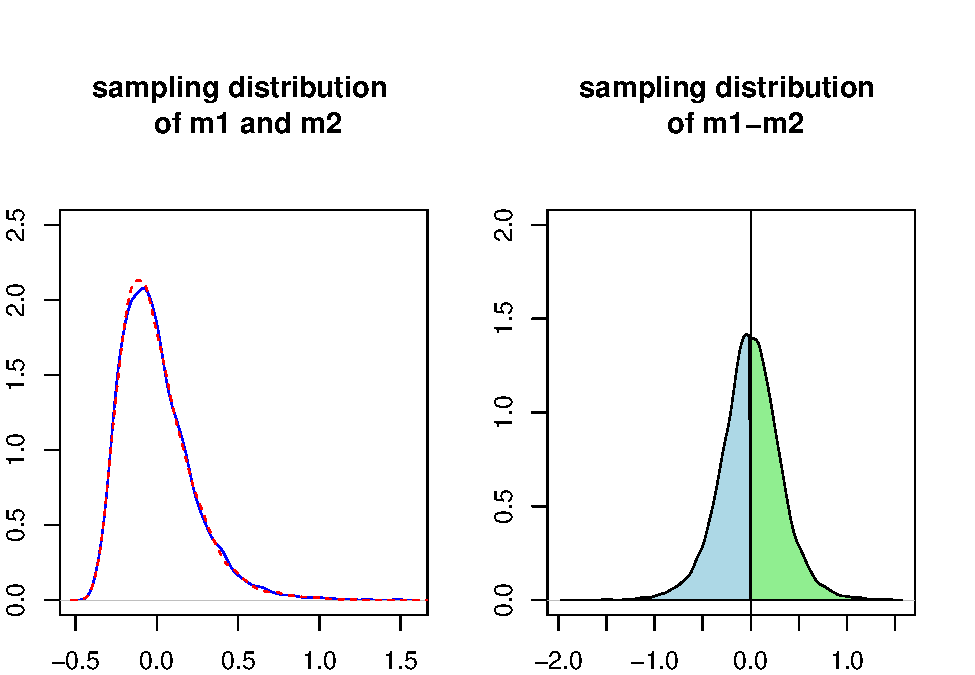
\includegraphics{Mathematical-study-of-Glass-s-d_files/figure-latex/sampldist1-1.pdf}
\caption{\label{fig:sampldist1}Sampling distribution of m1 (blue line in left plot), m2 (red dotted line in left plot), and m1-m2 (right plot), when m1 and m2 are estimates of the mean of a population distribution where mu=0, sigma=1,G1=6.32 and G2=95.75, with n1=n2=20}
\end{figure}

The sampling distributions of \(s_1\) and \(s_2\) are right-skewed, because estimates of the standard deviation are bounded: they can be very large, but never below 0. Moreover, as \(s_1\) and \(s_2\) are estimates of the same population standard deviation \(\sigma\), based on the same sample size, of course, the sampling distributions of \(s_1\) and \(s_2\) will be identical, as illustrated in Figure \ref{fig:sampldist2}.

\begin{figure}
\centering
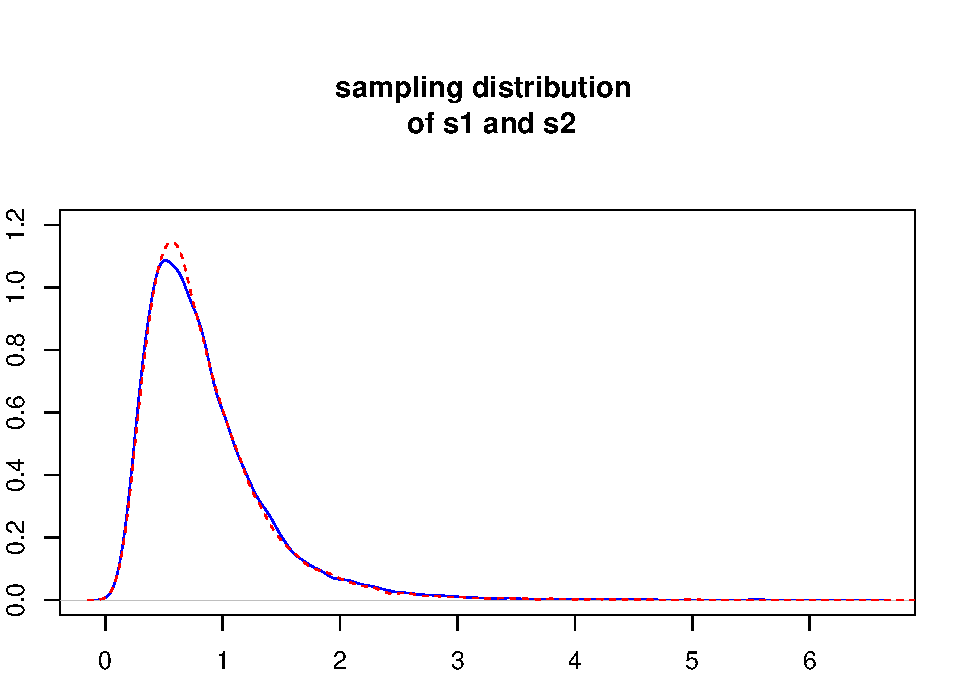
\includegraphics{Mathematical-study-of-Glass-s-d_files/figure-latex/sampldist2-1.pdf}
\caption{\label{fig:sampldist2}Sampling distribution of s1 (blue line) and s2 (red dotted line), when s1 and s2 are estimates of the standard deviation of a population distribution where mu=0, sigma=1,G1=6.32 and G2=95.75, with n1=n2=20}
\end{figure}

Therefore, how to explain the different sampling distributions of glass's \(d_s\), as a function of the standardizer? This is due to the fact that when distributions are skewed, there is a non-nul correlation between \(\bar{X}\) and s (see Zhang, 2007). More specifically, when distributions are right-skewed, there is a \textbf{positive} correlation between \(\bar{X}\) and s, as illustrated in the left plots in Figure \ref{fig:meanvssd1}.

\begin{figure}
\centering
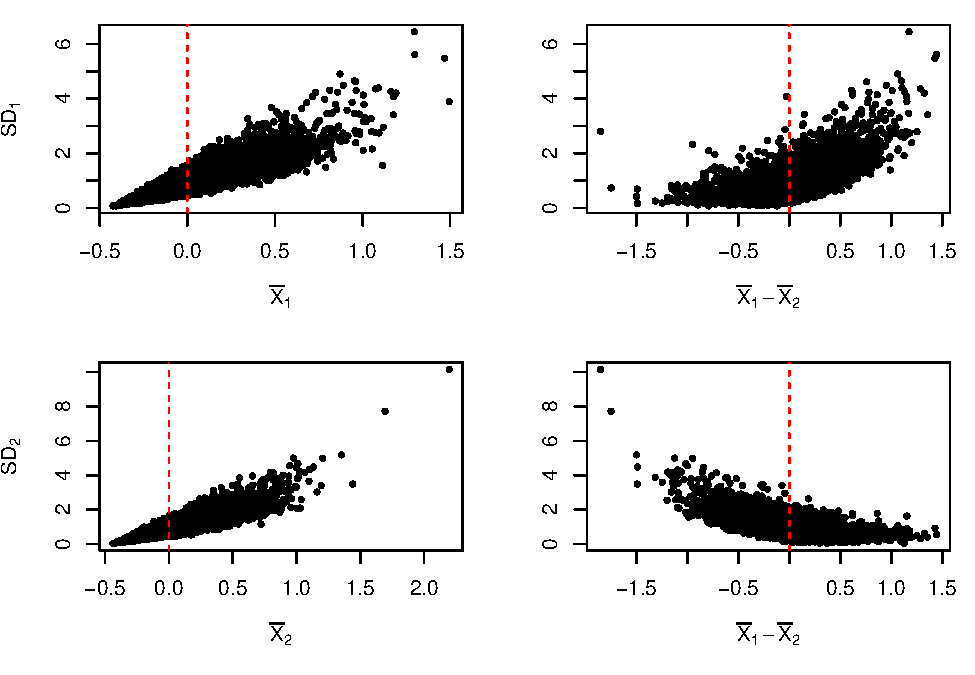
\includegraphics{Mathematical-study-of-Glass-s-d_files/figure-latex/meanvssd1-1.pdf}
\caption{\label{fig:meanvssd1}sample mean against sample standard deviation (left) and sample mean difference against sample standard deviation (right), for 100,000 iterations of sampling from two population distributions where mu=0, sigma=1,G1=6.32 and G2=95.75, with n1=n2=20}
\end{figure}

First, consider the glass's \(d_s\) estimate using \(s_1\) as standardiser. We already mentioned that there is a \emph{positive} correlation between \(\bar{X_1}\) and \(\bar{X_1}-\bar{X_2}\) (\(cor(\bar{X_1},\bar{X_1}-\bar{X_2})>0\)). Because there is also a positive correlation between \(\bar{X_1}\) and \(s_1\) (\(cor(\bar{X_1},s_1)>0\)), it results in a \textbf{positive} correlation between \(\bar{X_1}-\bar{X_2}\) and \(s_1\) (\(cor(\bar{X_1}-\bar{X_2},s_1)>0\); see top right plot in Figure \ref{fig:meanvssd1}): when moving from the left to the right in the right plot in Figure \ref{fig:sampldist1}, \(s_1\) get larger.

As a consequence, for many positive numbers k, \(-k\) will be divided by a smaller positive value (resulting in a larger ratio) than \(+k\), resulting in a left-skewed sampling distribution of glass's \(d_S\).\footnote{This is not true for each value of k, because the correlation between the mean difference and standard deviation estimates is not perfect, but the larger k (i.e. the more extreme the mean difference estimate), the larger the probability that it is true.} Importantly, while the median of the sampling distribution of glass's \(d_s\) is 0, as expected (because the sampling distributions of \(\bar{X_1}-\bar{X_1}\) is centered around 0), the mean will be a little lower (i.e.~-0.17), meaning that glass's \(d_s\) is negatively biased.

When considering \(s_2\) as standardiser, because there is a \emph{negative} correlation between \(\bar{X_2}\) and \(\bar{X_1}-\bar{X_2}\), there is also a \textbf{negative} correlation between \(\bar{X_1}-\bar{X_2}\) and \(s_2\) (see bottom right plot in Figure \ref{fig:meanvssd1}): when moving from the left to the right in the right plot in Figure \ref{fig:sampldist1}, \(s_2\) get lower. In other word, for many positive numbers k, \(-k\) will be divided by a larger positive value (resulting in a larger ratio) than \(+ k\), resulting in a right-skewed sampling distribution of glass's \(d_S\). This time, while the median of the sampling distribution of glass's \(d_s\) is still 0, the mean will be a little larger (i.e.~0.17), meaning that glass's \(d_s\) is positively biased.

\hypertarget{when-both-samples-are-extracted-from-a-common-left-skewed-distribution-mu_1-mu_20-top-left-plot-in-figure}{%
\subsection{\texorpdfstring{When both samples are extracted from a common left-skewed distribution (\textbf{\(\mu_1-\mu_2=0\)}) (top left plot in Figure \ref{fig:glass2})}{When both samples are extracted from a common left-skewed distribution (\textbackslash mu\_1-\textbackslash mu\_2=0) (top left plot in Figure )}}\label{when-both-samples-are-extracted-from-a-common-left-skewed-distribution-mu_1-mu_20-top-left-plot-in-figure}}

When distributions are left-skewed, one observes the opposite: there is a \textbf{negative} correlation between \(\bar{X}\) and s, as illustrated in the left plots in Figure \ref{fig:meanvssd2}.

\begin{figure}
\centering
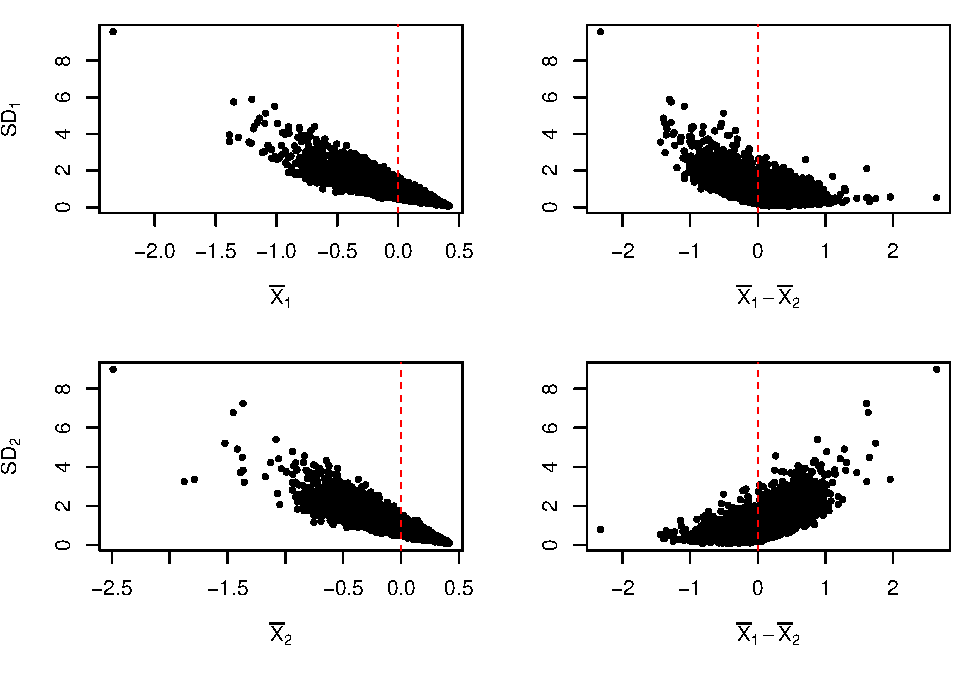
\includegraphics{Mathematical-study-of-Glass-s-d_files/figure-latex/meanvssd2-1.pdf}
\caption{\label{fig:meanvssd2}sample mean against sample standard deviation (left) and sample mean difference against sample standard deviation (right), for 100,000 iterations of sampling from two population distributions where mu=0, sigma=1,G1=-6.32 and G2=95.75, with n1=n2=20}
\end{figure}

and therefore, when moving from the left to the right in the right plot in Figure \ref{fig:sampldist1}, \(s_1\) get lower (\(cor(\bar{X_1},s_1) < 0 \; and \; cor(\bar{X_1},\bar{X_1}-\bar{X_2}>0) \rightarrow cor(\bar{X_1}-\bar{X_2},s_1)<0\)) and \(s_2\) get larger (\(cor(\bar{X_2},s_2) < 0 \; and \; cor(\bar{X_2},\bar{X_1}-\bar{X_2}<0) \rightarrow cor(\bar{X_1}-\bar{X_2},s_2)>0\)). As a consequence, glass's \(d_S\) will be positively biased when using \(s_1\) as a standardiser, and negatively biased when using \(s_2\) as a standardiser.

\hypertarget{when-samples-are-extracted-from-skewed-distributions-with-mu_1-mu_21-bottom-plot-in-figure}{%
\subsection{\texorpdfstring{When samples are extracted from skewed distributions, with \textbf{\(\mu_1-\mu_2=1\)} (bottom plot in Figure \ref{fig:glass2})}{When samples are extracted from skewed distributions, with \textbackslash mu\_1-\textbackslash mu\_2=1 (bottom plot in Figure )}}\label{when-samples-are-extracted-from-skewed-distributions-with-mu_1-mu_21-bottom-plot-in-figure}}

We will first consider the example where both samples are extracted from right-skewed distributions with \(\mu_1\) and \(\mu_2\) being respectively 1 and 0, and other moments of the population distributions being equal: \(\sigma=1\), \(\gamma_1=6.32\) and \(\gamma_2=95.75\) (see bottom right plot in Figure \ref{fig:glass2}).

Of course, the sampling distributions of \(\bar{X_1}\) and \(\bar{X_2}\) are not superimposed anymore, because \(\bar{X_1}\) will be centered around \(\mu_1=1\), and \(\bar{X_2}\) will be centered around \(\mu_2=0\). However, except for the mean, all other moments of both distributions (i.e.~\(\gamma_1\), \(\gamma_2\) and \(\sigma\)) remain identical (see left plot in Figure \ref{fig:sampldist4}) and therefore, the sampling distribution of \(\bar{X_1}-\bar{X_2}\) still follow a symmetric distribution, as illustrated in the right plot in Figure \ref{fig:sampldist4}.

\begin{figure}
\centering
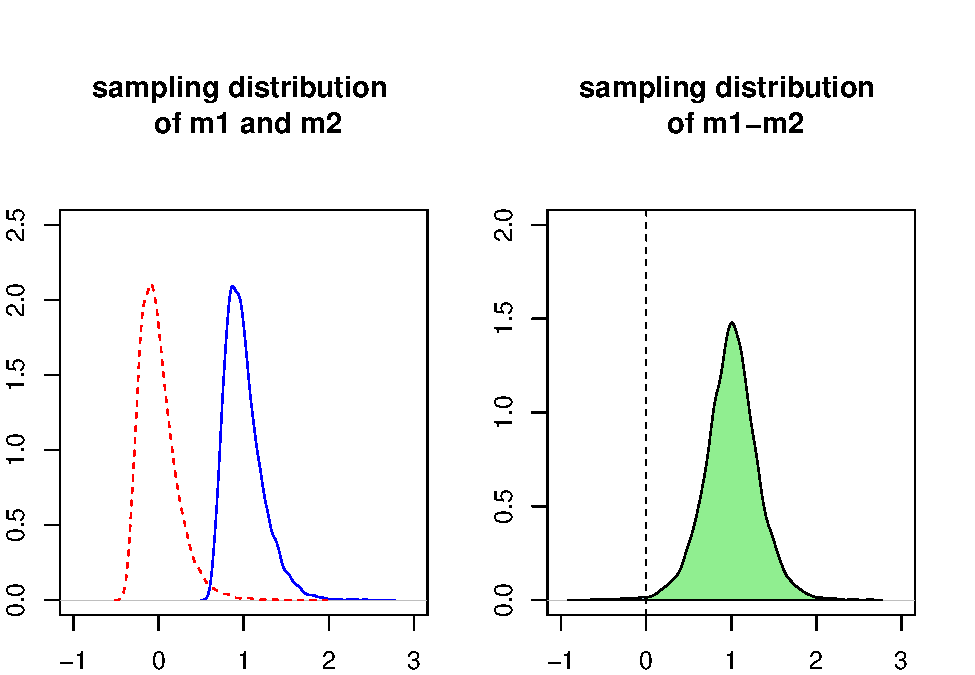
\includegraphics{Mathematical-study-of-Glass-s-d_files/figure-latex/sampldist4-1.pdf}
\caption{\label{fig:sampldist4}Sampling distribution of m1 (blue line in left plot), m2 (red dotted line in left plot), and m1-m2 (right plot), when m1 is the mean of a sample extracted from a population distribution where mu=1 and m2 is the mean of a sample extracted from a population distribution where mu2=0. Except for the mean, all other moments of both populations distributions are identical, i.e.~sigma=1,G1=6.32 and G2=95.75, with n1=n2=20}
\end{figure}

When \(\mu_1-\mu_2\) was nul, comparing the magnitude of glass's \(d_S\) when \(\bar{X_1}-\bar{X_2} = (\mu_1-\mu_2) \pm k\) was only a function of the denominator (as \(|(\mu_1-\mu_2)-k|=|(\mu_1-\mu_2)+k|\)). When \(\mu_1-\mu_2 \neq 0\), it is a function of both numerator and denominator. For example, when \(\mu_1-\mu_2=1\), only about 0.40\% of the mean estimates are negative, meaning that almost all mean difference estimates will be positive (so will be glass's \(d_s\) estimates). When computing glass's \(d_s\) using \(s_1\) as standardizer, the mean difference estimates that are close of 0 will be divided by a smaller standard deviation estimate that larger mean difference estimates (as \(cor(\bar{X_1}-\bar{X_2},s_1)>0\)). On the other side, when computing glass's \(d_s\) using \(s_2\) as standardizer, the mean difference estimates that are very small will be divided by a larger standard deviation estimate than large mean difference estimates (as \(cor(\bar{X_1}-\bar{X_2},s_2)<0\)). It is therefore not surprising that the sampling distribution of glass's \(d_s\) is more skewed and variable when using \(s_2\) rather than \(s_1\) as standardizer.\footnote{Of course, when the mean difference is negative, this is the opposite: the sampling distribution of glass's $d_s$ will be left-skewed, and will be more skewed and variable when using $s_1$ rather than $s_2$ as standardizer}. When distributions are extracted from a left-skewed distribution (bottom left in Figure \ref{fig:glass2}), this is exactly the opposite.

\hypertarget{when-two-samples-are-extracted-from-distributions-with-identical-shapes-and-n_1-neq-n_2}{%
\section{\texorpdfstring{When two samples are extracted from distributions with identical shapes, and \(n_1 \neq n_2\)}{When two samples are extracted from distributions with identical shapes, and n\_1 \textbackslash neq n\_2}}\label{when-two-samples-are-extracted-from-distributions-with-identical-shapes-and-n_1-neq-n_2}}

When population distributions are symmetric (i.e.~\(\gamma_1=0\)), the sampling distribution of glass's \(d_s\) is only a function of the sample size of the group from which standardizer is computed (because \(\sigma_1=\sigma_2\)). Using the SD of the smallest group as standardiser results in a more biased and variable measure of Glass's \(d_S\), whatever it is the first or the second group, as illustrated in Figure \ref{fig:glass3}.

\begin{figure}
\centering
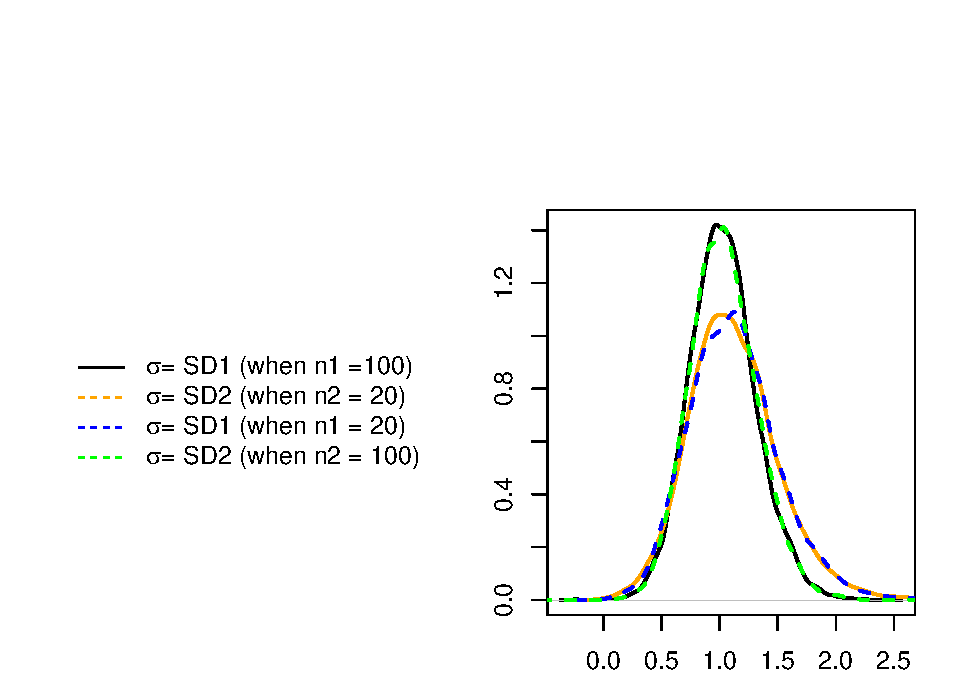
\includegraphics{Mathematical-study-of-Glass-s-d_files/figure-latex/glass3-1.pdf}
\caption{\label{fig:glass3}Comparison of Glass's ds when choosing either sd1 or sd2 as standardizer when both samples are extracted from a distribution where sigma=1, m1=1,m2=0, G1=0 and G2=95.75, and either n1=100 and n2=20, or n1=20 and n2=100}
\end{figure}

We know that the sampling distribution of \(\bar{X_1}-\bar{X_2}\) is always symmetric, but that the sampling distribution of any standard deviation is right-skewed (because a standard deviation can never be below 0). The lower the sample size, the more skewed the sampling distribution of the standard deviation and the larger it's variance. As a consequence, the more skewed the sampling distribution of glass's \(d_s\)).

When distributions are skewed, the skewness of the glass's \(d_s\) distribution (and therefore, the bias and variance of glass's \(d_s\)) depends on two parameters: the size of the group from which standardizer is computed (as with symmetric distributions), but also the correlation between \(\bar{X_1}-\bar{X_2}\) and \(s_j\). As long as \(\mu_1-\mu_2\) is positive (or negative), the more skewed and variable estimation of glass's \(d_s\) will occur when \(s_j\) is simultaneously negatively (or positively) correlated with \(\bar{X_1}-\bar{X_2}\) and computed based on the smallest sample size. On the other side, the best estimation (less biased and variable) will occur when \(s_j\) is simultaneously positively (or negatively) correlated with \(\bar{X_1}-\bar{X_2}\) and computed based on the largest sample size. This is illustrated in Figure \ref{fig:glass4} in four plots where samples are extracted from either a right-skewed distribution (\(\gamma_1=6.32\); right) or a left-skewed distribution (\(\gamma_1=-6.32\); left), and with a positive (top) or negative (bottom) population mean difference.

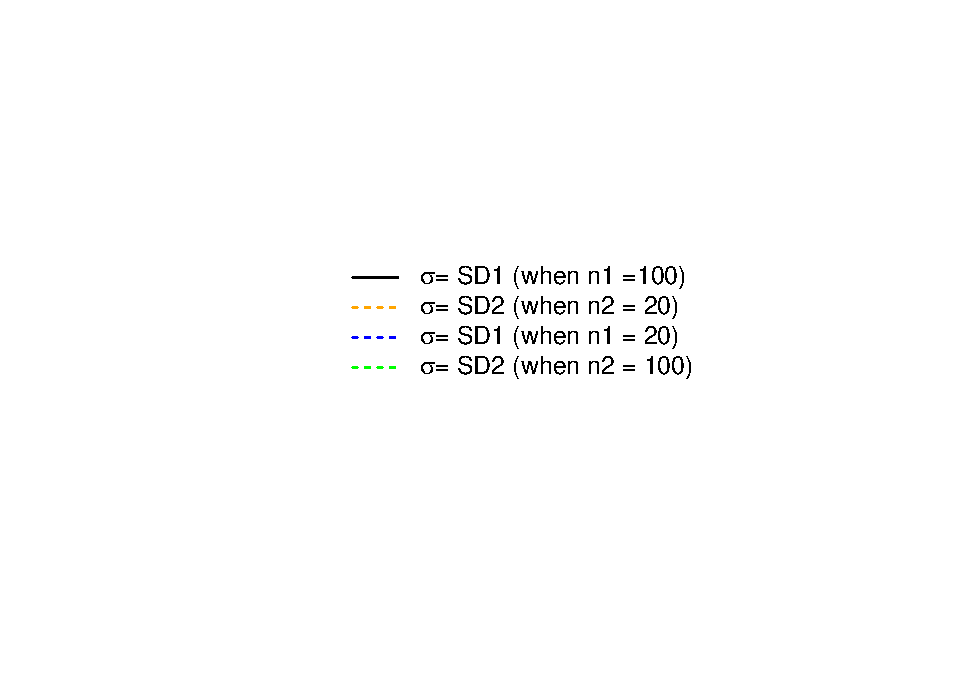
\includegraphics{Mathematical-study-of-Glass-s-d_files/figure-latex/legend-1.pdf}

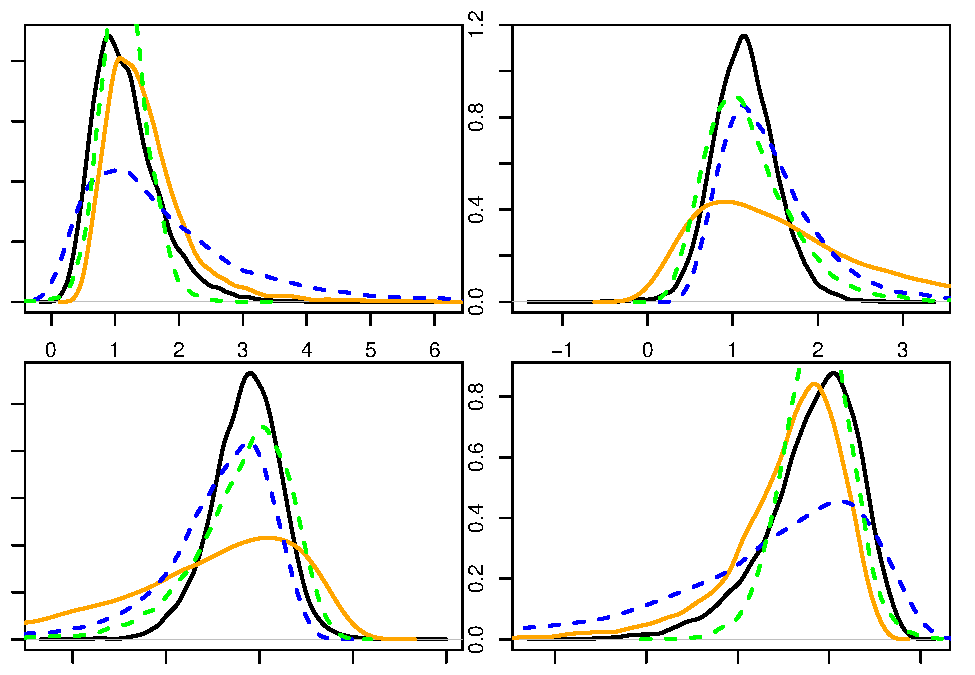
\includegraphics{Mathematical-study-of-Glass-s-d_files/figure-latex/glass4-1.pdf}
In the two top plots in Figure \ref{fig:glass4}, \(\bar{X_1}-\bar{X_2}\) is positive. When distributions are right-skewed (top right), choosing \(s_2\) (i.e.~the \(SD\) that is negatively correlated with \(\bar{X_1}-\bar{X_2}\)) associated with the smallest sample size (i.e.~\(n_2=20\)) will result in the most biased and variable estimation of glass's \(d_s\). The best estimation will occur when choosing \(s_1\) associated with the largest sample size (i.e.~\(n_1=100\)). On the other side, when distributions are left-skewed (top left), choosing \(s_1\) (i.e.~the \(SD\) that is negatively correlated with \(\bar{X_1}-\bar{X_2}\)) associated with the smallest sample size (i.e.~\(n_1=20\)) will result in the most biased and variable estimation of glass's \(d_s\). The less biased and variable glass \(d_s\) will occur when \(s_2\) is chosen as standardizer and \(n_2=100\).

In the two bottom plots in Figure \ref{fig:glass4}, \(\bar{X_1}-\bar{X_2}\) is negative. When distributions are right-skewed (bottom right), choosing \(s_1\) (i.e.~the \(SD\) that is positively correlated with \(\bar{X_1}-\bar{X_2}\)) associated with the smallest sample size (i.e.~\(n_1=20\)) will result in the most biased and variable estimation of glass's \(d_s\). The best estimation will occur when choosing \(s_2\) associated with the largest sample size (i.e.~\(n_2=100\)). On the other side, when distributions are left-skewed (top left), choosing \(s_2\) (i.e.~the \(SD\) that is positively correlated with \(\bar{X_1}-\bar{X_2}\)) associated with the smallest sample size (i.e.~\(n_2=20\)) will result in the most biased and variable estimation of glass's \(d_s\). The less biased and variable glass \(d_s\) will occur when \(s_1\) is chosen as standardizer and \(n_1=100\).

Note: when computing an effect size estimates where standardizer is computed based on both \(SD_1\) and \(SD_2\), the correlation between standardizer and \(\bar{X_1}-\bar{X_2}\) is null.

\hypertarget{when-two-samples-are-extracted-from-distributions-with-identical-shapes-with-sigma_1-neq-sigma_2-and-n_1n_2}{%
\section{\texorpdfstring{When two samples are extracted from distributions with identical shapes, with \textbf{\(\sigma_1 \neq \sigma_2\)} and \textbf{\(n_1=n_2\)}}{When two samples are extracted from distributions with identical shapes, with \textbackslash sigma\_1 \textbackslash neq \textbackslash sigma\_2 and n\_1=n\_2}}\label{when-two-samples-are-extracted-from-distributions-with-identical-shapes-with-sigma_1-neq-sigma_2-and-n_1n_2}}

It is interesting to study the sampling distribution of s, \(\bar{X_1}-\bar{X_2}\) and glass's \(d_s\) (using either \(SD_1\) or \(SD_2\) as standardiser), as a function of \(\sigma\), for different kind of distributions, and more specifically, the variance of their sampling distribution.

The larger \(\sigma\), the larger the standard deviation of \(\bar{X_1}-\bar{X_2}\). In the left plot in Figure \ref{fig:meandiffbis}, we plotted \(sd(\bar{X_1}-\bar{X_2})\) against \(\sigma\) for different kind of distributions underlying the data. We can see that the standard deviation of the sample mean difference does not depend on the distribution (it is the same for all represented distributions underlying the data). However, it is always a function of \(\sigma\), as we can see in the right plot in Figure \ref{fig:sdsamplbis}, where we plotted \(\frac{sd(\bar{X_1}-\bar{X_2})}{\sigma}\). This value is constant for any value of \(\sigma\).

\begin{figure}
\centering
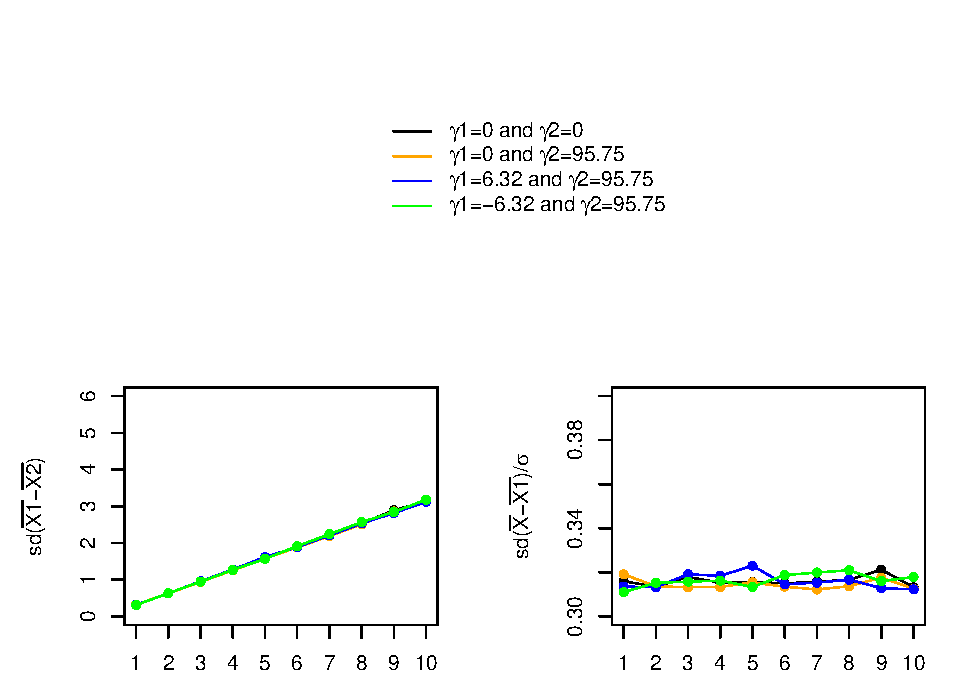
\includegraphics{Mathematical-study-of-Glass-s-d_files/figure-latex/meandiffbis-1.pdf}
\caption{\label{fig:meandiffbis}standard deviation of the sampling distribution of s, as a function of sigma, for difference distributions underlying the data}
\end{figure}

As for the sample mean difference, the larger \(\sigma\), the larger the standard deviation of the sampling distribution of \(s\). In the left plot in Figure \ref{fig:sdsamplbis}, we plotted \(sd(s)\) against \(\sigma\) for different kind of distributions underlying the data. We can see that unlike the standard deviation of \(\bar{X_1}-\bar{X_2}\), the standard deviation of \(S\) is larger when distributions are symmetric with high kurtosis than when distributions are normal, and that the variance of \(s\) is even larger when distributions are skewed. Again, it is also always a function of \(\sigma\), as we can see in the right plot in Figure \ref{fig:sdsamplbis}, where we plotted \(\frac{sd(s)}{\sigma}\). This value is constant for any value of \(\sigma\).

\begin{figure}
\centering
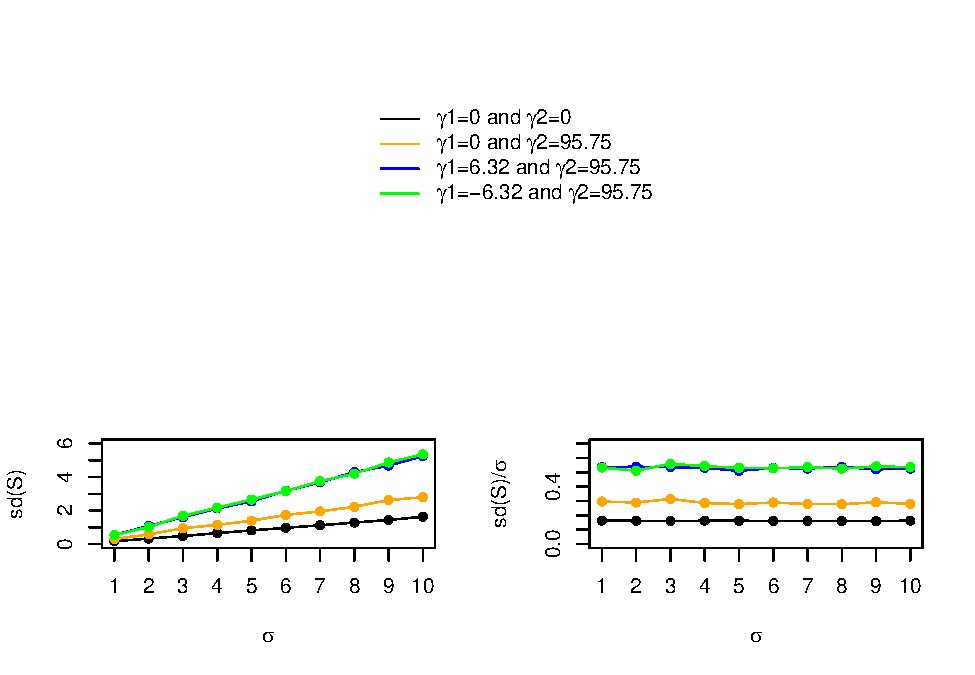
\includegraphics{Mathematical-study-of-Glass-s-d_files/figure-latex/sdsamplbis-1.pdf}
\caption{\label{fig:sdsamplbis}standard deviation of the sampling distribution of s, as a function of sigma, for difference distributions underlying the data}
\end{figure}

\begin{figure}
\centering
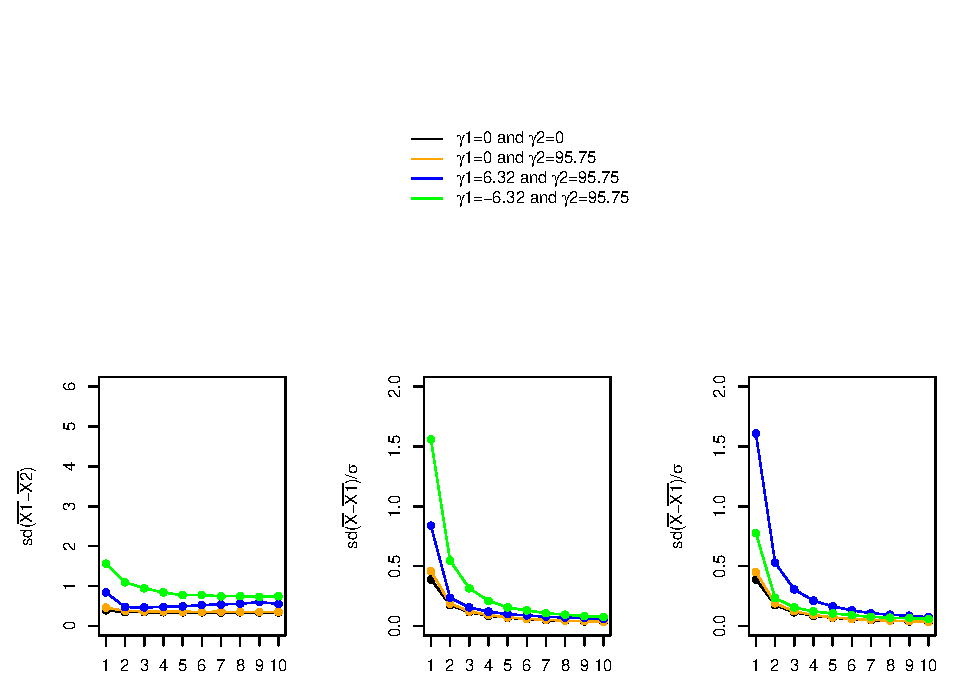
\includegraphics{Mathematical-study-of-Glass-s-d_files/figure-latex/ratiosamplbis-1.pdf}
\caption{\label{fig:ratiosamplbis}standard deviation of the sampling distribution of s, as a function of sigma, for difference distributions underlying the data}
\end{figure}

\begin{figure}
\centering
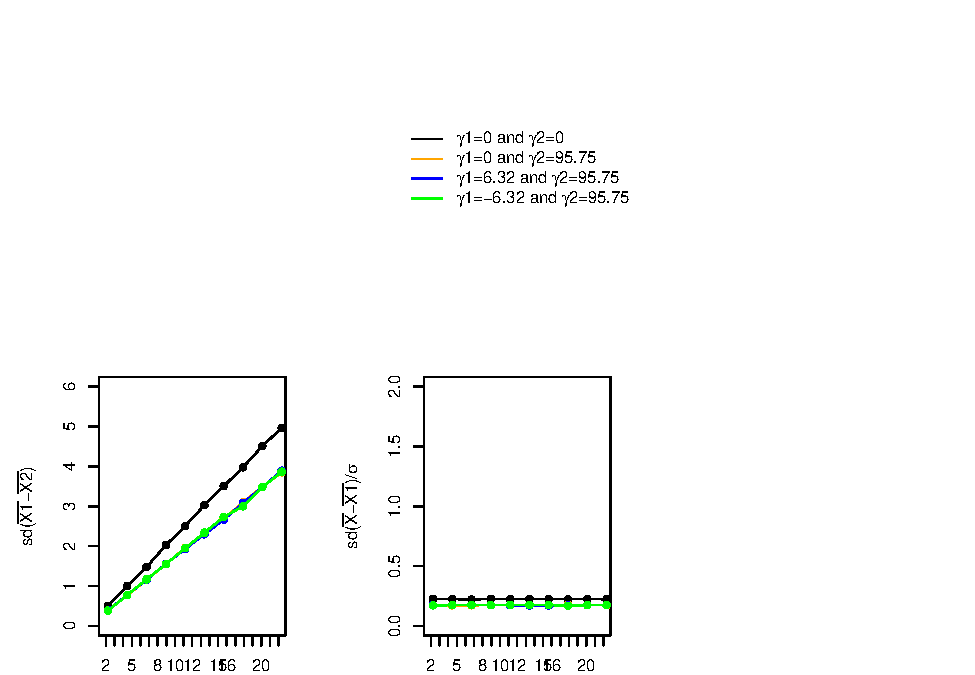
\includegraphics{Mathematical-study-of-Glass-s-d_files/figure-latex/meandiffter-1.pdf}
\caption{\label{fig:meandiffter}standard deviation of the sampling distribution of s, as a function of sigma, for difference distributions underlying the data}
\end{figure}

Rem que pour le test, j'avais reproduit le script mais pour voir le sd d'une moyenne d'échantillon, et comme pour la différence de moyenne, ça ne dépend PAS de la distribution (strange, mais c'est comme ça).

\begin{itemize}
\tightlist
\item
  L'écart-type de la distribution d'échantillonnage de la moyenne ne dépend PAS de la distribution (ce n'est qu'une fonction de sigma)
\item
  L'écart-type de la distribution d'échantillonnage de SD dépend d la distribution par contre!
\end{itemize}

\end{document}
